\documentclass{scrreprt}
\usepackage[english]{babel}
\usepackage[T1]{fontenc}
\usepackage{lmodern}
\usepackage{blindtext}
\usepackage[utf8]{inputenc}
\usepackage{siunitx} %For unit handling%
\renewcommand{\familydefault}{\sfdefault}
\newcommand{\unit}[1]{\ensuremath{\, \mathrm{#1}}}
\usepackage{amssymb, amsmath, cancel, ulem, graphicx, float, tabularx, multirow, bm}
\usepackage{amsmath}
\usepackage{caption}
\usepackage{subcaption}
\usepackage{mathtools}
\usepackage{tikz}
\usepackage{commath}
\newcommand*\circled[1]{\tikz[baseline=(char.base)]{
            \node[shape=circle,draw,inner sep=1pt] (char) {#1};}}
\renewcommand{\phi}{\varphi}


\setcounter{secnumdepth}{5}
\setcounter{tocdepth}{5}

\author{Urs Gerber\\09-921-156 \and Gian-Luca Mateo\\11-113-545}
\date{25th of April 2013}

\title{Spectrometer}
\subtitle{Practical course report}

\begin{document}

\maketitle

\tableofcontents
\newpage

\chapter{Experiment: Spectrometer}

\section{Introduction}

\subsection{Goal of the experiment}
The goal of this experiment is to analyze the visible light spectrum of a mercury vapor lamp. To do this a spectrometer is first calibrated and then used to find the angles of refraction along the edge of a prism made of glass for a certain wavelength. In addition, we examine some physical properties of the spectrometer's prism.
 
\subsection{Theory}
\subsubsection{Spectrometer}
A spectrometer is a device which is used to examine the spectral composition of light emitted my a certain material. It's functionality is based on the fact that the refractive index $n$ of a material is depending on the wavelength $\lambda$ of the incoming light beam. This effect is called \emph{dispersion relation} and is illustrated in figure \ref{fig:dispersion}.\\

\begin{figure}[h]
	\centering
  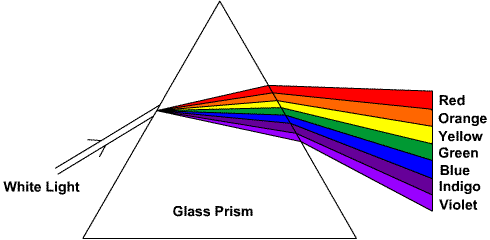
\includegraphics[width=0.5\textwidth]{img/dispersion.png}
	\caption{Dispersion along the edge of a glass prism}
	\label{fig:dispersion}
\end{figure}

One goal of this experiment is to characterize the prism of such a spectrometer. Opposite to the functionality mentioned above, the spectrometer can also be used to find the refractive index of the incoming at a certain wavelength by measuring the angle of deflection of the beam after travelling through the prism. In order to do that, the minimum angle of deflection $\delta_m$ must be found for a given wavelength. This is the angle at which the spectrum reverses its direction, meaning that the spectrum is steady when the minimum angle of deflection is reached. At this angle, the following relation holds:

\begin{equation}\label{eq:index}
n = \frac{\sin\alpha_1}{\sin\beta_1} = \frac{\sin{\left(\frac{\delta_m+\phi}{2} \right)}}{\sin{\frac{\phi}{2}}}
\end{equation}

where $\alpha_1$ is the angle of incidence, $\beta_1$ the angle of reflection and $\phi$ the prism's wedge angle. This relation will be used to calculate the refractive indices of the prism at different wavelengths.\\

Additionally, if the prism's base length $a$ is known, the resolution $A$ of the prism can be found by using the derivative of the refractive index with respect to the wavelength $\frac{\dif n}{\dif \lambda}$:

\begin{equation}\label{eq:resolution_calc}
A = a\cdot \frac{\dif n}{\dif \lambda}
\end{equation}

The minimal resolution to be able to distinguish two spectral lines can be found via 

\begin{equation}\label{eq:resolution_theory}
A_{\text{Theory}} = \frac{\lambda}{\Delta \lambda}
\end{equation}

\subsubsection{Spectral lines of mercury}

The observed spectral lines of mercury are listed below in table \ref{tab:spectral_lines}

\begin{table}[H]
\centering
\begin{tabular}{|l|c|}
\hline
Color & wave length $\lambda$ [nm]\\
\hline\hline
dark red & 690.8\\
red & 623.4 \\
yellow I & 579.1\\
yellow II & 577.0\\
green & 546.1\\
blue-green & 491.6\\
indigo & 435.8\\
purple I & 407.8\\
purple II & 404.7\\\hline
\end{tabular}
\caption{Spectral lines of mercury}
\label{tab:spectral_lines}
\end{table}

To determine the minimal base length $a$ necessary at which the two yellow spectral lines can still be visually distinguished can be found by mounting a variable slit of width $x$ in front of the objective. Using 

\begin{equation}\label{eq:slit}
x = \frac{a}{2} \frac{\cos{\alpha_2}}{\sin{\frac{\phi}{2}}}
\end{equation}

and

\begin{equation}
\alpha_2 = \frac{\delta_m + \phi}{2} \quad ( = \alpha_1 \quad \text{at min. angle of deflection})
\end{equation}

we are able to calculate afore-said minimal base length $a$. 

\subsection{Error analysis}
The most interesting and relevant part of the error analysis is the one for the refractive index $n$ (angles in degrees):

\begin{equation}
s_n^2 = \frac{-s_{\delta_m}^2 (1+\cos{(\delta_m + \phi))} + s_{\phi}^2 ((-1+\cos \delta_m) \csc^2(\phi / 2))}{4 (-1 + \cos \phi)}
\end{equation}


\section{Experiment setup and execution}

\subsection{Used materials}
The materials used in this experiment are the following:
\begin{itemize}
\item a turntable, with an adjustable platform for the prism
\item a prism
\item a mercury vapor lamp
\item a collimator, mounted to the turntable, turnable 
\item a telescope, mounted to the turntable, turnable
\item an adjustable slit, mountable to the telescope
\end{itemize}

\subsection{Assembly and Execution}

\begin{figure}[H]
	\centering
  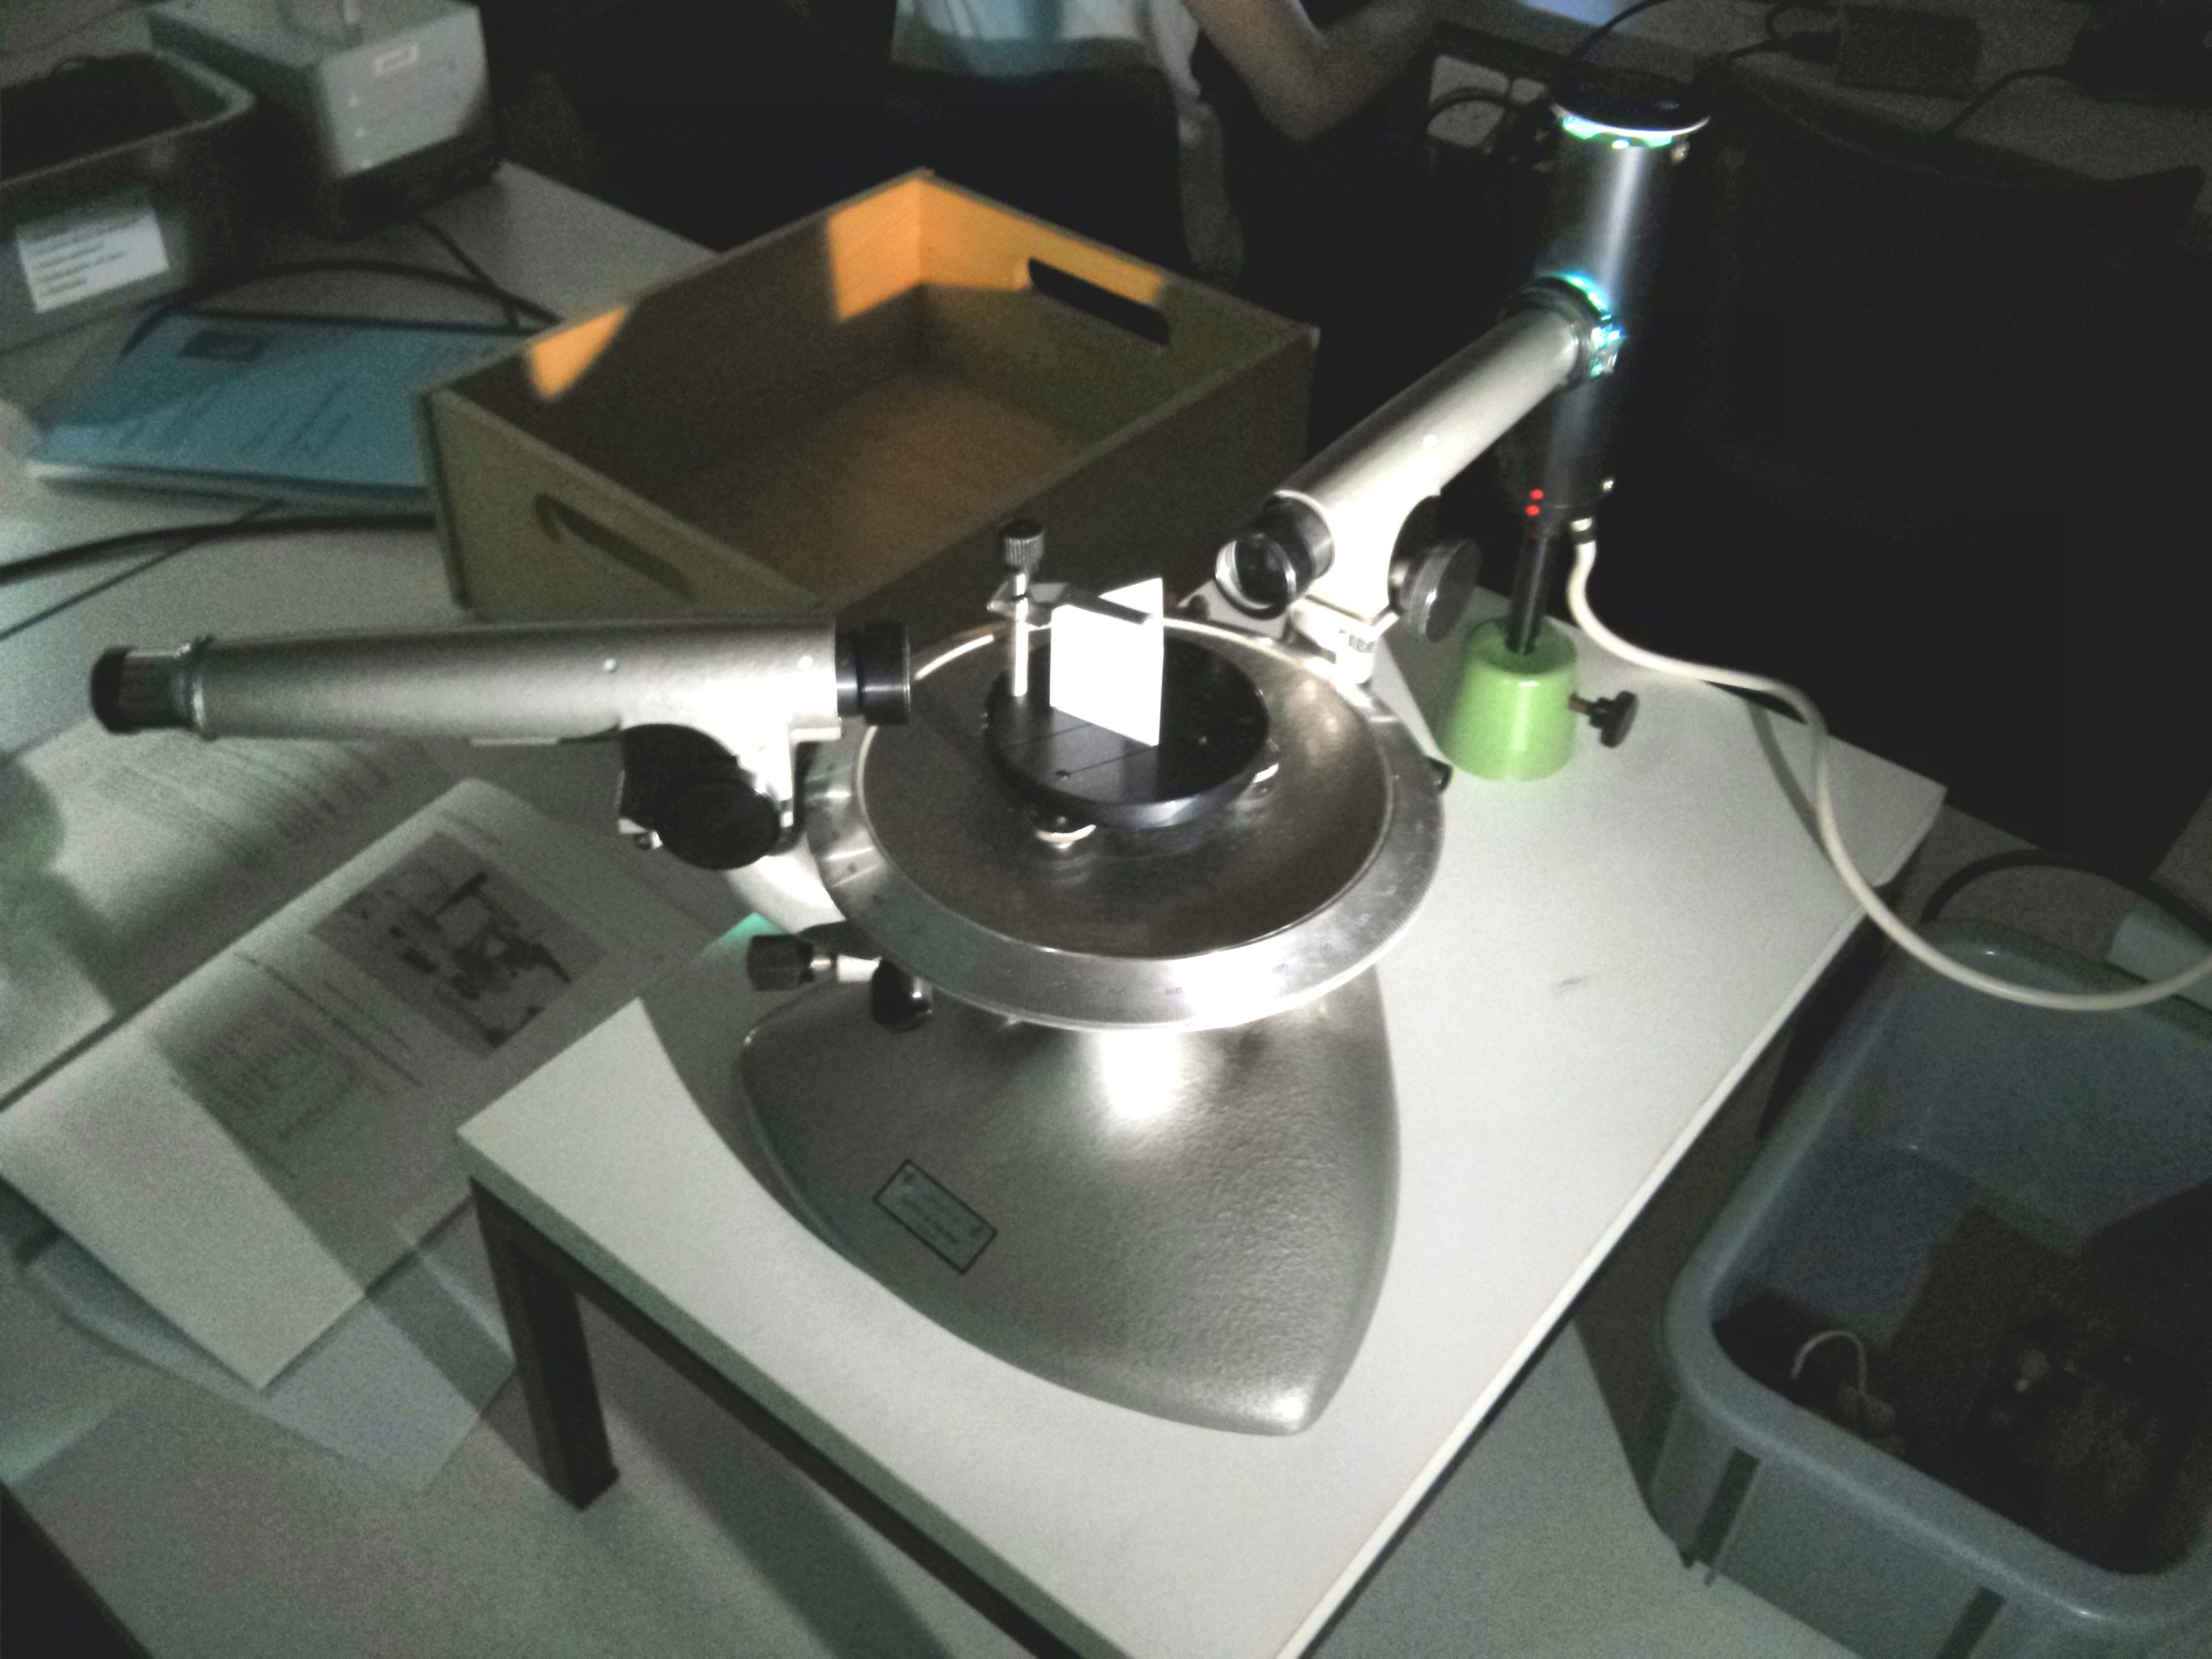
\includegraphics[width=0.9\textwidth]{img/assembly.jpg}
	\caption{Experiment Assembly}
	\label{fig:assembly}
\end{figure}

In the first measurement, we first adjusted the platform so the sides of the prism were exactly upright. Then, rotating the table to a position where one side faced the telescope, measuring the angle of the telescope and repeating the procedure for a second side, we measured the angle of the prism.
\\\\
For the second measurement, we lit up the vapor lamp and, rotating the platform, looked for the point where the spectral lines were minimally deflected. We measured that angle for each of the seven spectral lines stated in \cite[p. 159]{physcript13}. 
\\\\
For the third measurements, we mounted the adjustable slit on the telescope and closed it to the narrowest possible position where the yellow lines were still distinguishable, thus measuring the minimal base length. 
\section{Measurements}

\subsection{Minimal deflection}
\begin{figure}[H]
	\centering
  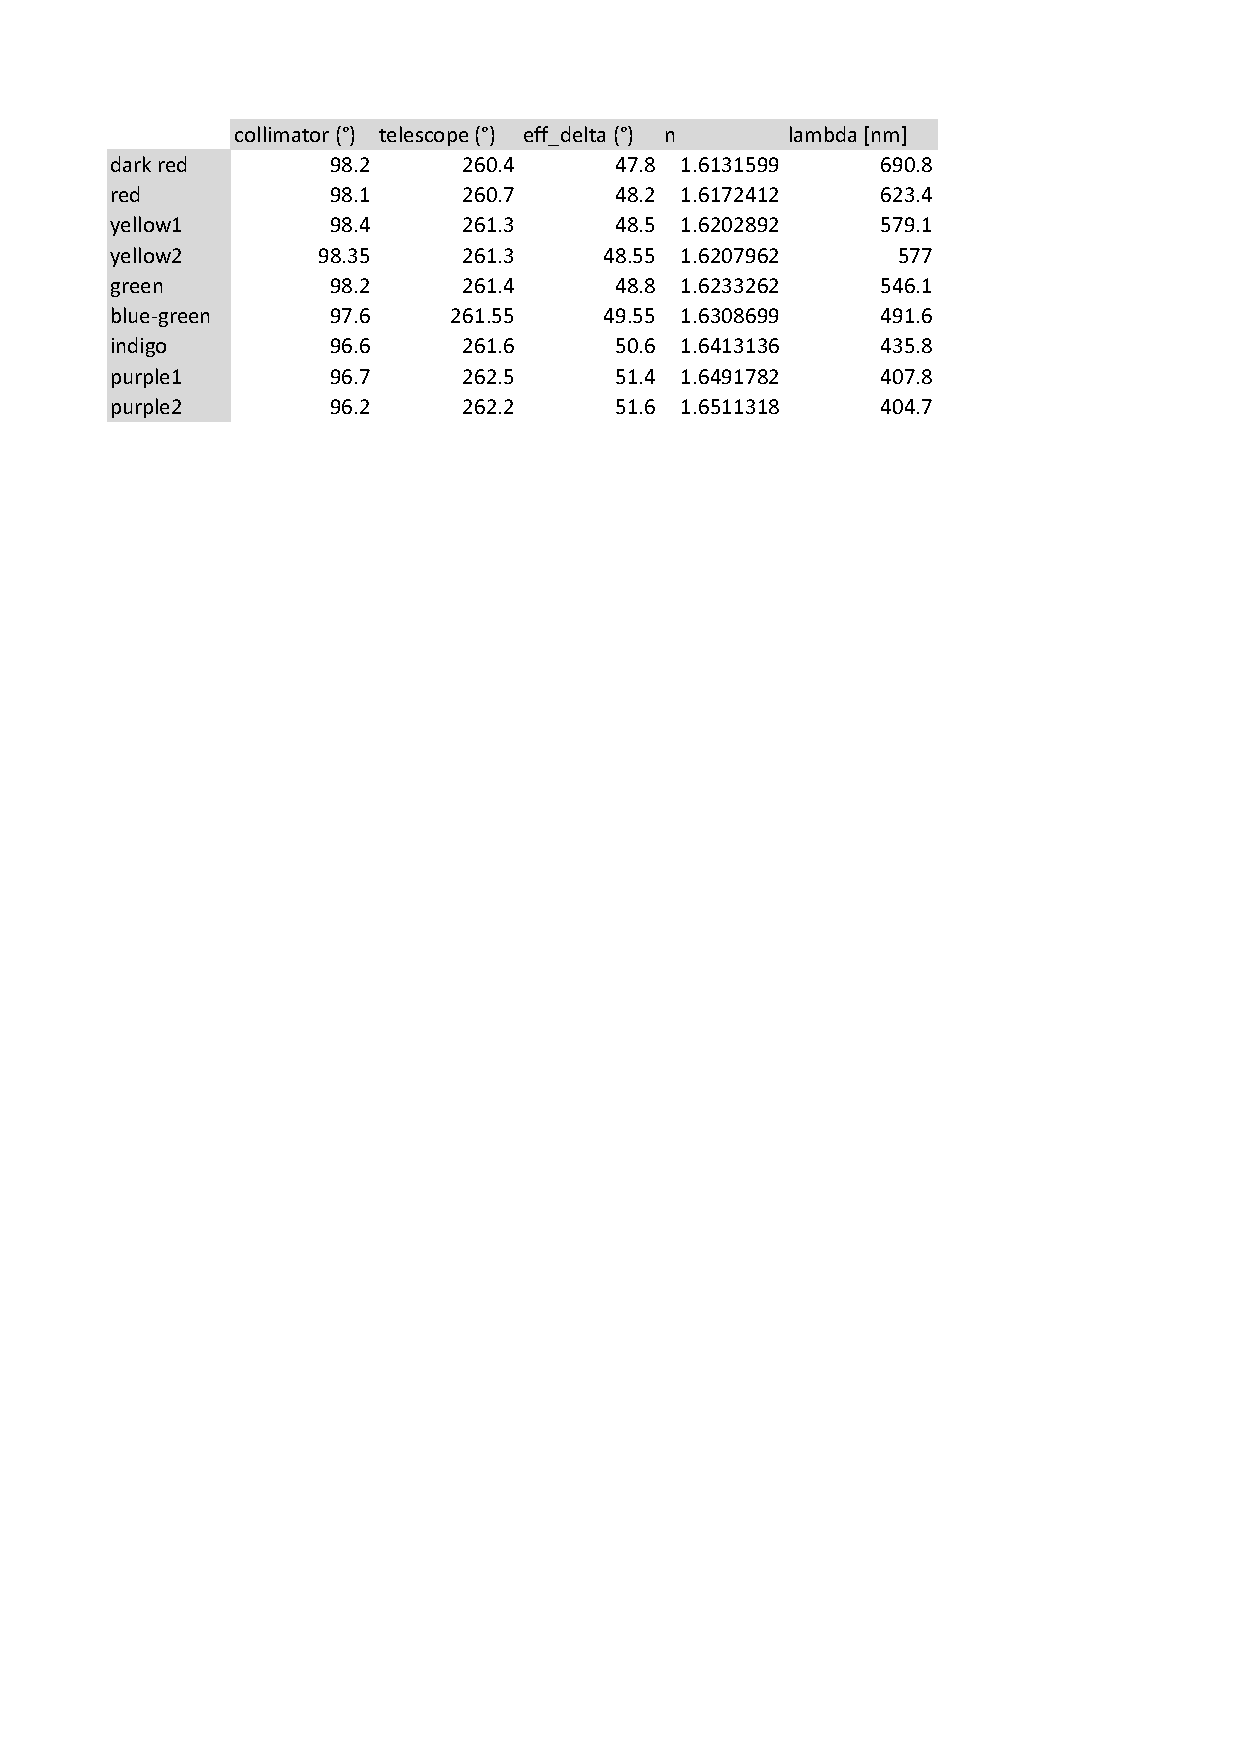
\includegraphics[width=0.9\textwidth]{diag/right.pdf}
	\caption{Minimum deflection angles on the right side}
	\label{fig:right}
\end{figure}

\begin{figure}[H]
	\centering
  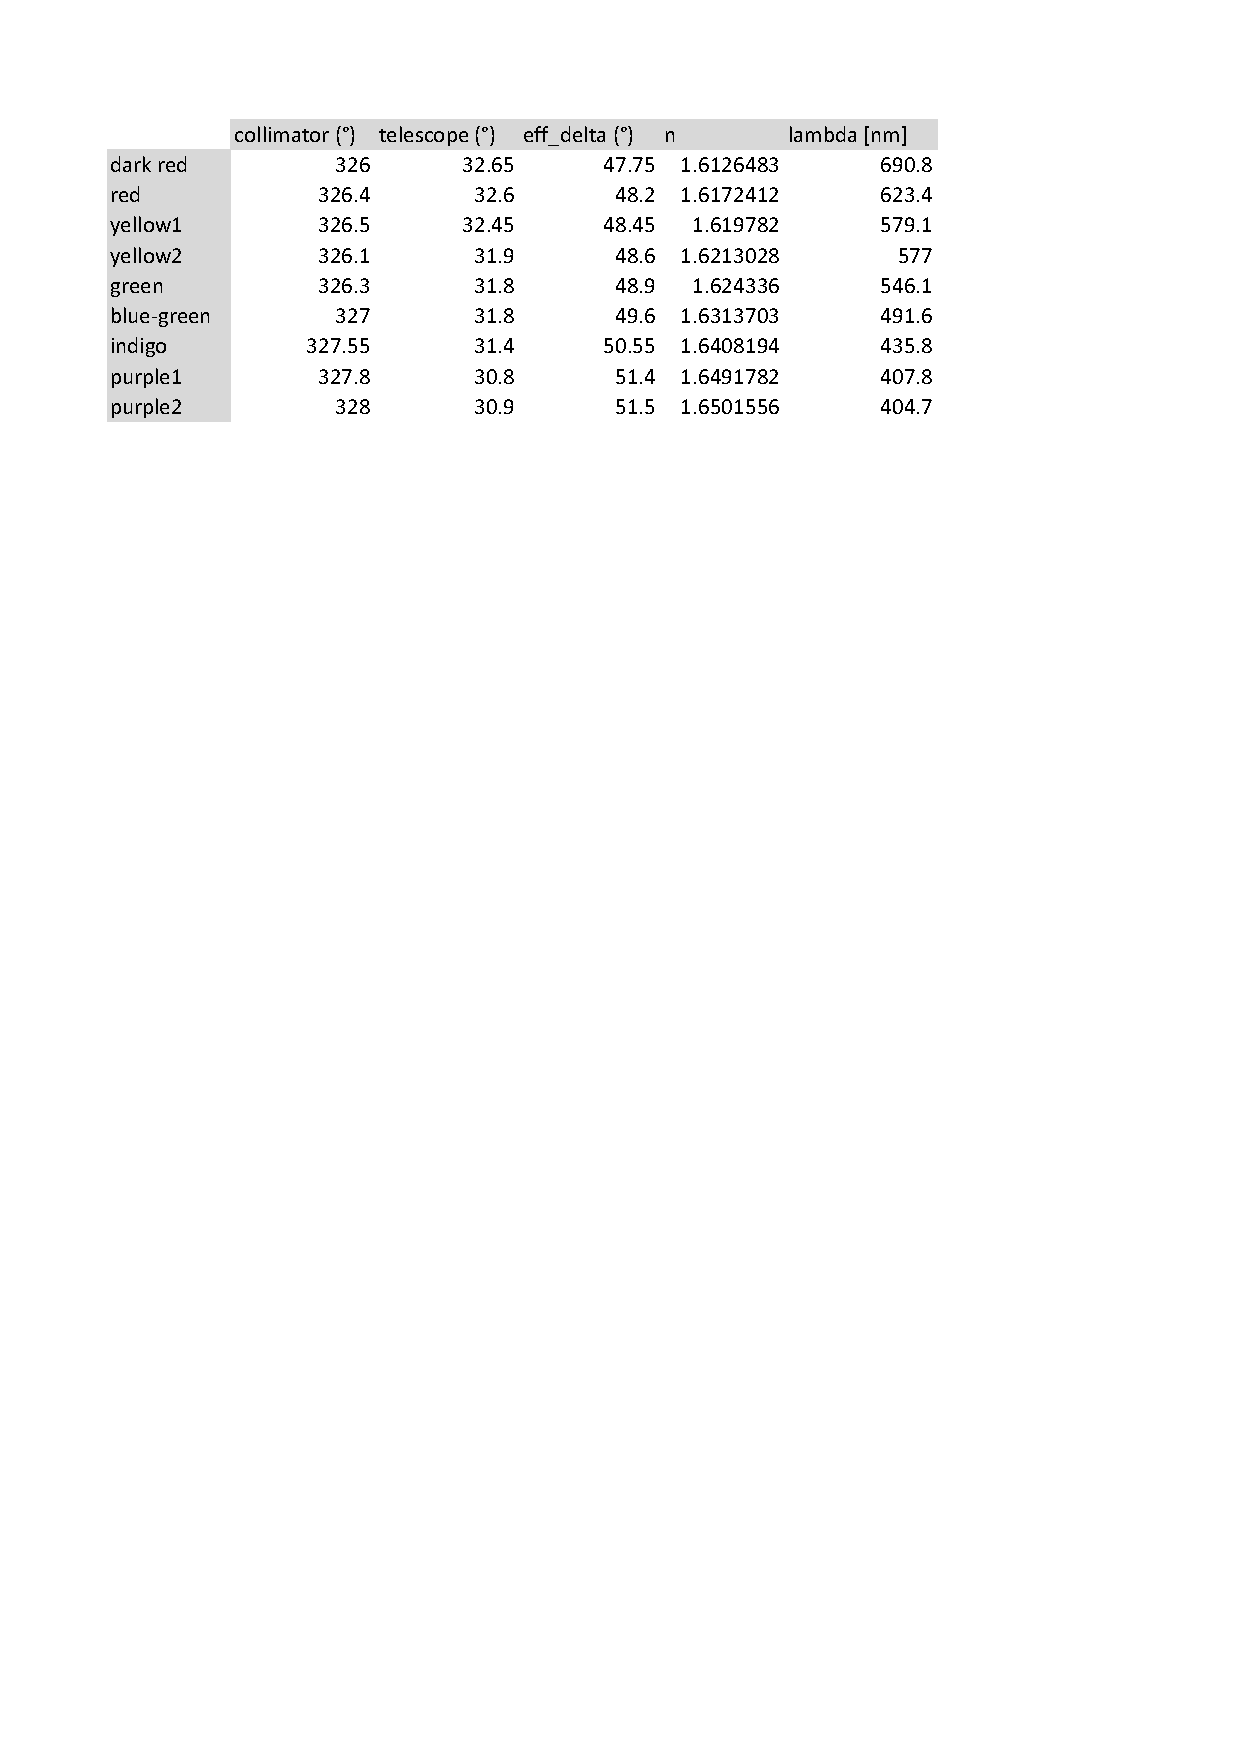
\includegraphics[width=0.9\textwidth]{diag/left.pdf}
	\caption{Minimum deflection angles on the left side}
	\label{fig:left}
\end{figure}
\subsection{Minimal Base Length}
We measured a minimal slit width $x$ of:
\begin{equation}
	x = 0.76\unit{mm}
\notag
\end{equation}

\section{Analysis and Discussion}

\subsection{Wedge Angle of the Prism}

Our measurements for the wedge angle of the prism yielded the following:
\begin{equation}
	\phi = \ang{60.2}
\notag
\end{equation}
We think the footprint of the used prism is an equilateral triangle, although we have no coherent experimental proof -- apart from our impression during the experiment --  for our assumption.

\subsection{Minimal Deflection}

Our measurements yield the following results:

\begin{table}[H]
\centering
\begin{tabular}{|l|c|c|c|}
\hline
Color & wave length $\lambda$ [nm] & $\delta_m$ [$^\circ$] & refractive index $n$\\
\hline\hline
dark red & 690.8 & $47.775 \pm 0.025$  & $1.613 \pm 0.000869$\\
red & 623.4 & $48.2 \pm 0.05$ & $1.617 \pm 0.000872$\\
yellow I & 579.1 & $48.475 \pm 0.025$ & $1.620 \pm 0.000874$\\
yellow II & 577.0 & $48.575 \pm 0.025$ & $1.621 \pm 0.000875$\\
green & 546.1 & $48.85 \pm 0.05$ & $1.624 \pm 0.000877$\\
blue-green & 491.6 & $49.575 \pm 0.025$ & $1.631 \pm 0.000883$\\
indigo & 435.8 & $0.575 \pm 0.025$ & $1.641 \pm 0.000891$\\\
purple I & 407.8 & $51.4 \pm 0.05$ & $1.649 \pm 0.000897$\\
purple II & 404.7 & $51.55 \pm 0.05$ & $1.651 \pm 0.000899$\\\hline
\end{tabular}
\caption{Refractive indices $n$ and minimum deflection angles $\delta_m$ at different wavelengths $\lambda$}
\label{tab:n_results}
\end{table}

The variable refractive indices $n$ are plotted against the wavelength $\lambda$ in figure \ref{fig:meas_and_fit} including a fit for our data points.

\begin{figure}[H]
	\centering
  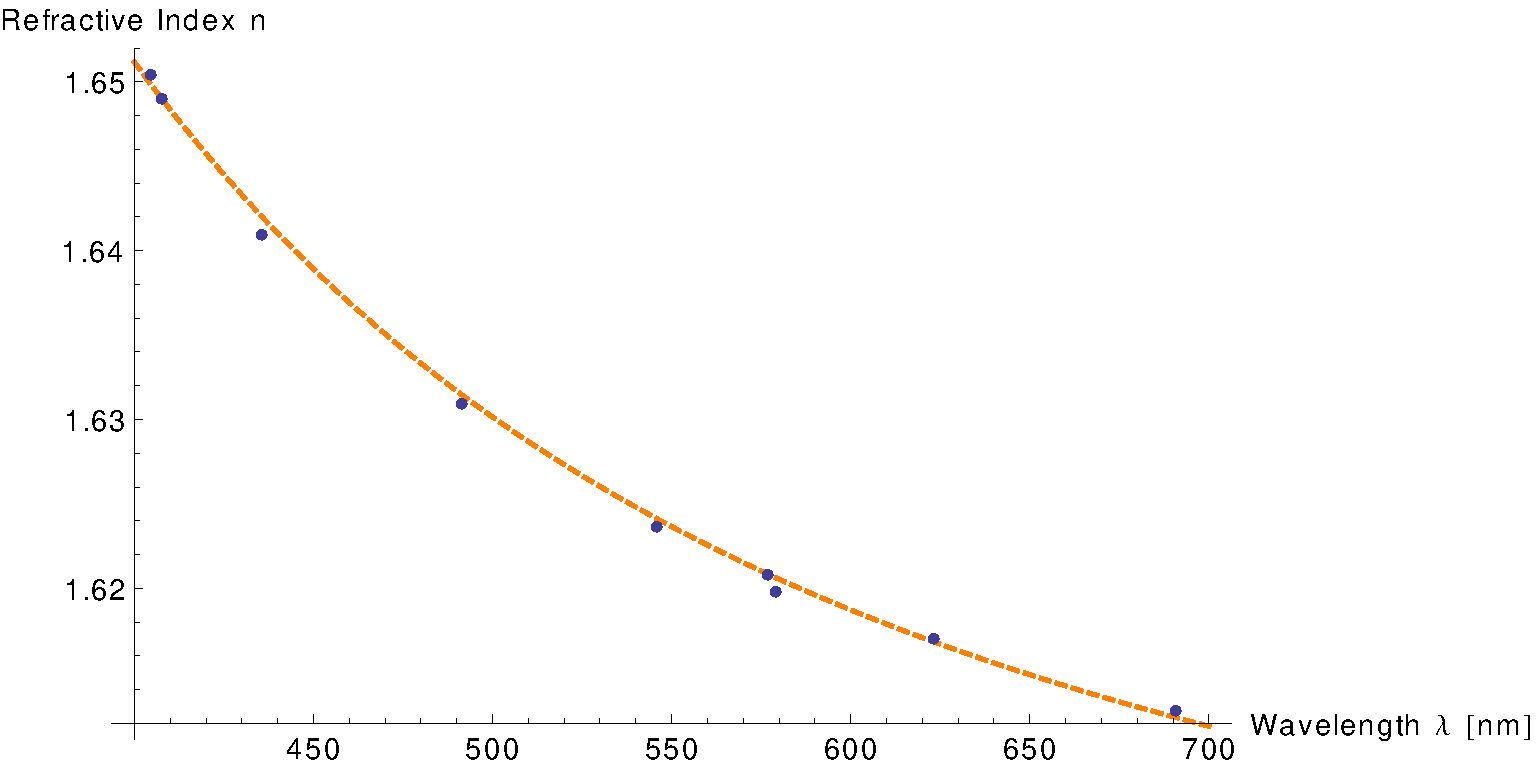
\includegraphics[width=0.9\textwidth]{diag/meas_and_fit.pdf}
	\caption{Calculated refractive indices $n$ plotted against the wavelength $\lambda$ of the spectrum with a fit (orange)}
	\label{fig:meas_and_fit}
\end{figure}
As predicted by theory, the refractive Index $n$ is higher for lower wavelengths and lower for higher wavelengths. Furthermore, the obtained values fall in line with values for different kinds of glass, which we think is a strong indication that our values are reasonable.\\

To be able to reasonably calculate the dispersion $\frac{\dif n}{\dif \lambda}$ for the task yet to come, we have created a mathematical model and let a computer find the best fit for our data and that particular model.

We found the model 
\begin{equation}
n (\lambda) = \frac{C}{\lambda^2}+k
\end{equation}
to be a reasonable approximation of our data points. Using Mathematica we could pinpoint both $C$ and $k$ (using a least squares algorithm) and the final approximation is

\begin{equation}\label{eq:approx}
n (\lambda) = \frac{9347.3}{\lambda^2}+1.59276
\end{equation} 

\subsection{Minimal Base Length}
\label{sec:base_length}

Using formula \ref{eq:slit} and the slit width $x$ determined in our measurements we can determine the minimal base length of a prism:
\begin{equation}
	a = 2 \cdot x \cdot \frac{\sin(\frac{\phi}{2})}{\cos({\alpha_2})} = 1.31 \unit{mm}	
\end{equation}
We decided to take this value with a grain of salt, as we could barely distinguish the yellow lines with our prism, which was distinctively larger. Then again, maybe a more powerful telescope would have helped.

\subsection{Resolution}
Using formula \ref{eq:resolution_calc} and using $\frac{\dif{n}}{\dif{\lambda}}$ of our fit \ref{eq:approx} at $\lambda = 578.05 \unit{nm}$, which is between the yellow spectral lines, we calculated the resolution of our prism:
\begin{equation}
	A_{\text{meas}} = 2622.944
	\notag
\end{equation}
If we compare that to the theoretically necessary resolution:
\begin{equation}
	A_{\text{theory}} = 275.262
	\notag
\end{equation}
We see that our resolution is substantially larger than needed according to theory. This result falls in line with the one obtained in \ref{sec:base_length} and indicates that a smaller prism would have sufficed to distinguish the yellow spectral lines. If we solve formula \ref{eq:resolution_calc} for $a$ we can get another value for the minimal base length and compare it to the one obtained in \ref{sec:base_length}.
\begin{equation}
	a_{res} = A_{theory} \cdot \left(\frac{\dif{n}}{\dif{\lambda}}\right)^{-1} = 2.844 \unit{mm}
\notag
\end{equation}
Considering that we used the derivation of a numerical fit, the results support the validity of our calculations in \ref{sec:base_length}.

\subsubsection{Sources of error}
In about every step we took when setting up and running the experiment we ran into a whole set of small and more profound difficulties. First, the calibration of the spectrometer could not be perfectly carried out, as the turntable could not be fixed without interfering with the setup of the other devices. Also, we found our prism not to be a perfectly equilateral, but in most cases this effect is nullified by incorporating the actual angles in our measurements. The prism was not absolutely clean either, probably because of previous groups touching it with their greasy fingers.
Furthermore, the collimator and telescope probably were not adjusted to the maximum possible precision.\\
The most profound source of error in our view is the human eye. After observing an object from such a short distance for a long time, it gets increasingly difficult to distinguish spectral lines that are very close to each other. 

\section{Conclusion}

\begin{thebibliography}{9}

\bibitem{physcript13}
  Peter Wurz,
  \emph{Anleitung zum Physikpraktikum}
  FS2013

\end{thebibliography}

\end{document}
